\section{Stochastic Secretary Problem}
\label{stochastic_k_secretary}
\cut{
\begin{figure}
 %\vspace{-5pt}
    \centering
    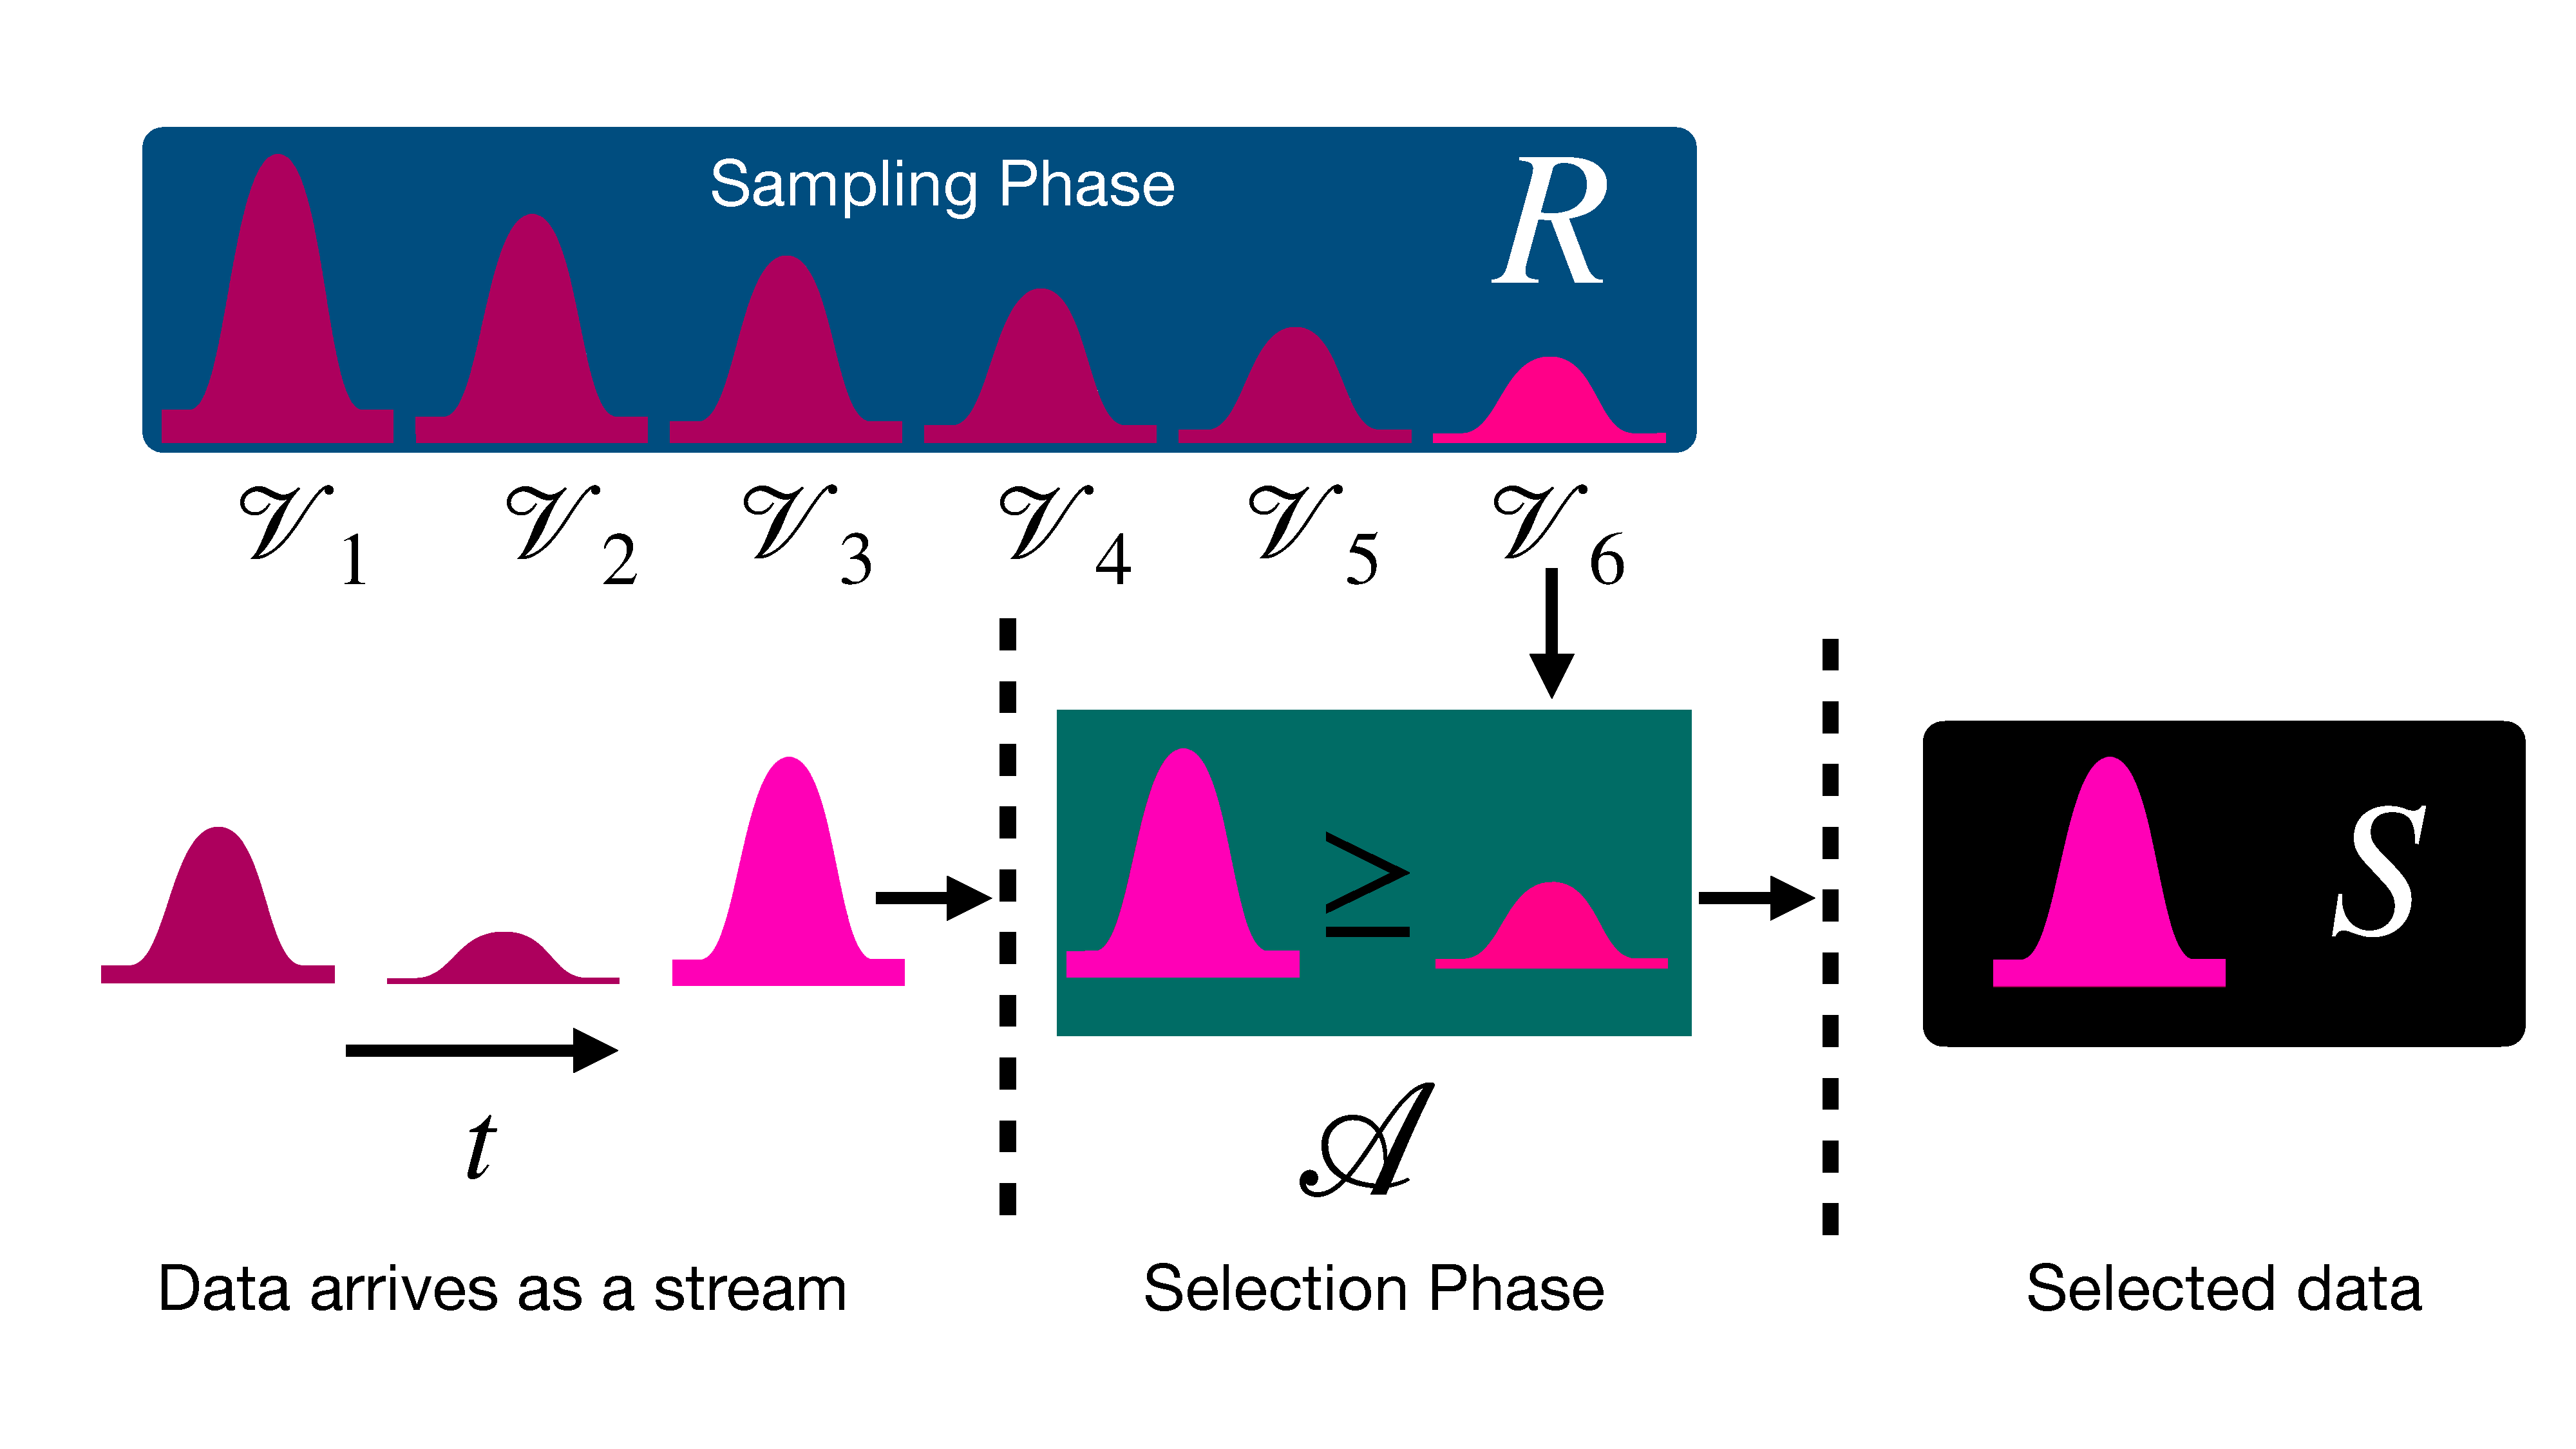
\includegraphics[width=0.48\linewidth]{Figures/stochastic_secretary_fixed.pdf}
    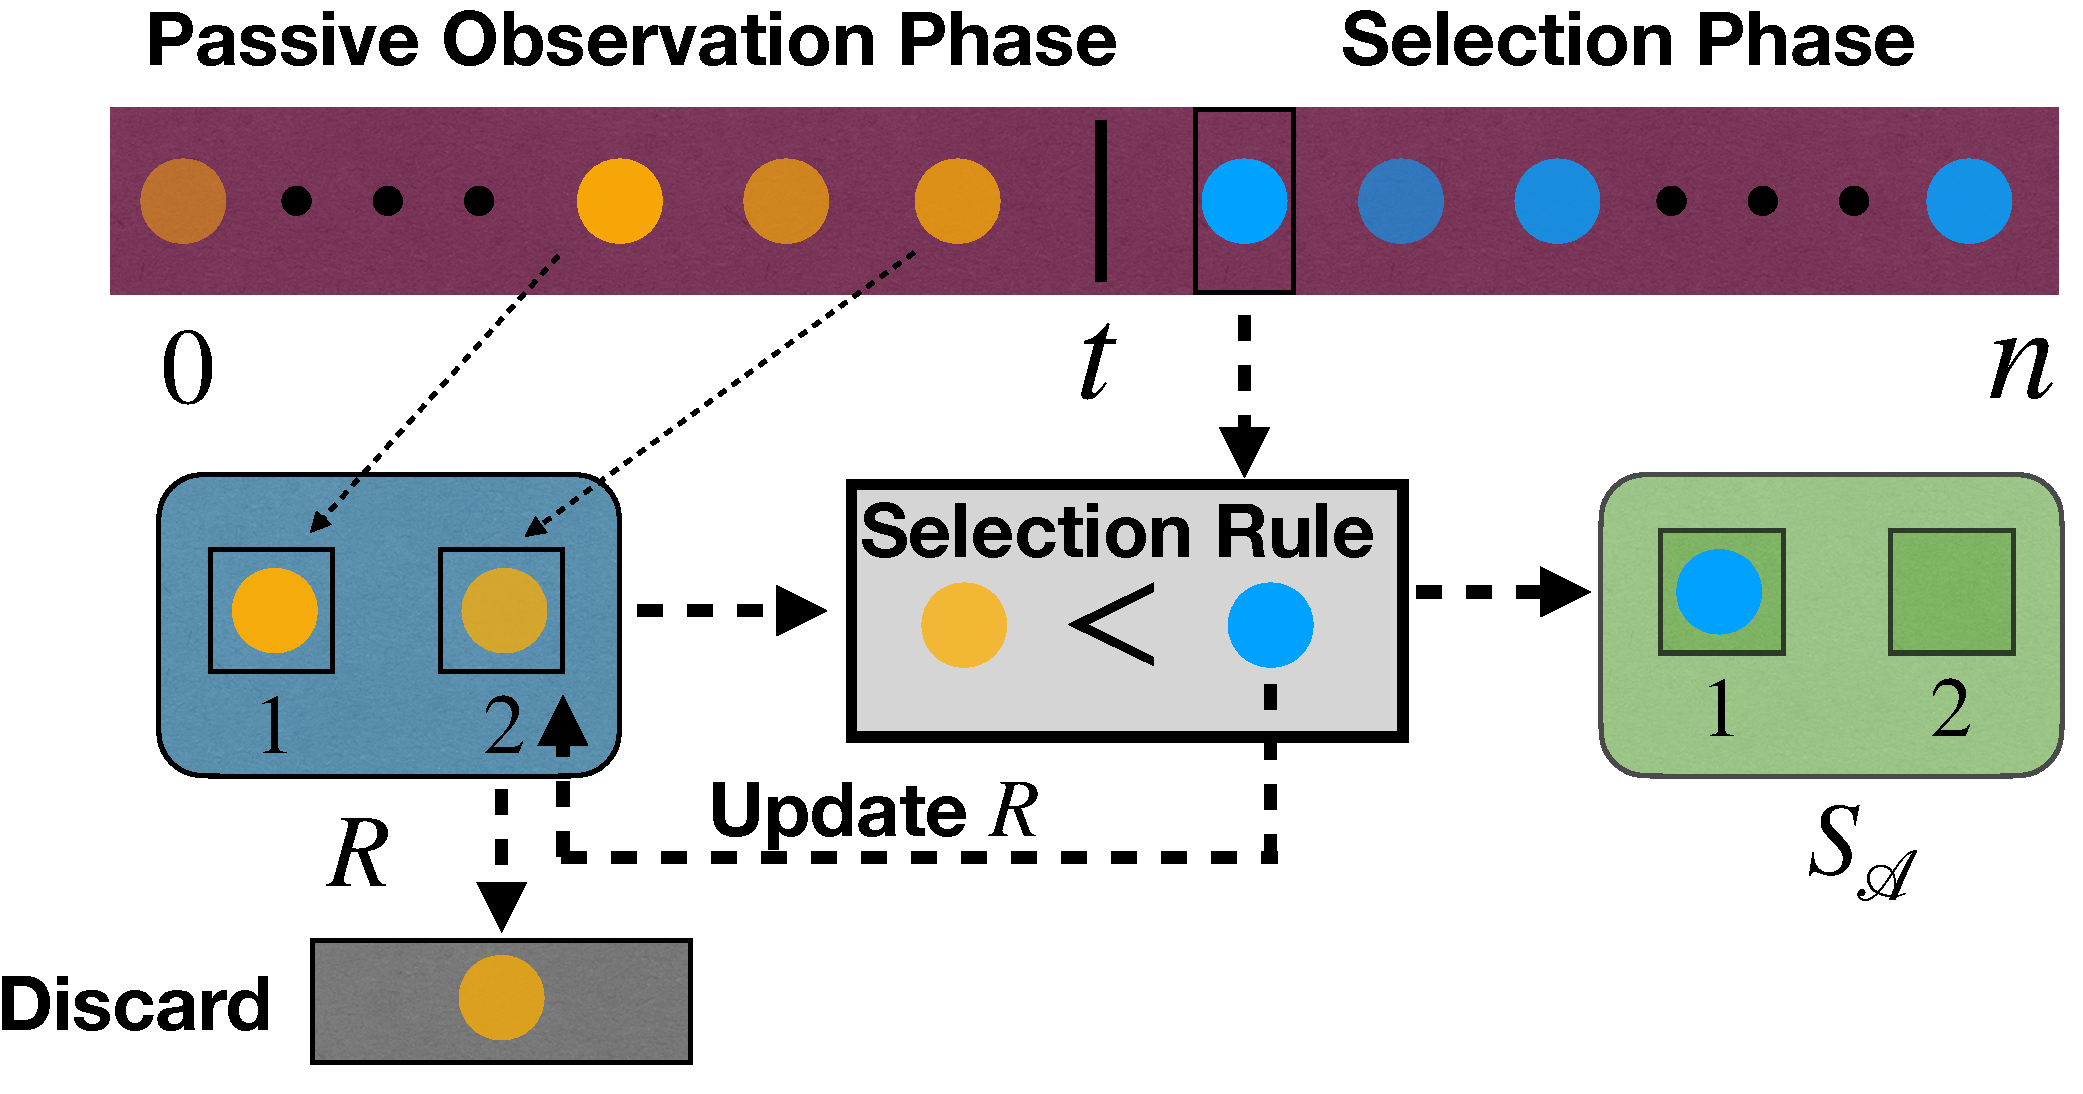
\includegraphics[width=0.48\linewidth]{Figures/Virtual+_algo.pdf}
    %\vspace{-10pt}
    \caption{Each online algorithm, $\mathcal{A}$, observes estimates of $v_i$ and maintains a reference list $R$ during the sampling phase. Items are then picked into $S_{\mathcal{A}}$, after threshold $t$, via comparisons to $R$.}
    \label{fig:stochastic_secretary}
\end{figure}
}
In practice, online adversaries are unlikely to have access to the target model $f_t$.
Instead, it is reasonable to assume that they have partial knowledge. 
%ut instead some partial knowledge. Examples of partial knowledge that have been studied in the blackbox setting include forming input-output queries \cite{ilyas2017query,ilyas2018black,ilyas2018prior} for iterative refinement of an attack vector. However, these sources of knowledge are no longer conducive in the online setting due to transiency of data and we do not consider them. 
Following \cite{papernot2016practical,bose2020adversarial} we focus on modeling that partial knowledge by equipping the adversary with a surrogate model or representative classifier $f_s$. Using $f_s$ as opposed to $f_t$ means that we can compute the value $\mathcal{V}_i:= \ell(f_s(x_i'),y_i)$ of an incoming data point. This value $\mathcal{V}_i$ acts as an estimate of the value of interest $v_i:=\ell(f_t(x_i'),y_i)$. The {\em stochastic $k$-secretary problem} is then to pick, under the noise model induced by using $f_s$, the optimal subset $S_{\mathcal{A}}$ of size $k$ from $\mathcal{D}$. 
Thus, with no further assumptions on $f_s$ it is unclear whether online algorithms, as defined in ~\S\ref{virtual_plus}, are still serviceable under uncertainty.

\xhdr{Sources of randomness}
Our method relies on the idea that we can use the surrogate model $f_s$ to estimate the value of some adversarial examples on the target model $f_t$. We justify here how partial knowledge on $f_t$ could provide us an estimate of $v_i$.
For example, we may know the general architecture and training procedure of $f_t$, but there will be inherent randomness in the optimization (e.g., due to initialization or data sampling), making it impossible to perfectly replicate $f_t$. 
Consequently, we can view the training of a surrogate model $f_s$---using the same general training procedure---as a sample from a common (for $f_s$ and $f_t$) underlying distribution $\mathcal T$. In that context, it seems reasonable to assume that the random variable $\mathcal{V}_i := \ell(f_s(x'_i),y_i)$ is likely to be close to $v_i := \ell(f_t(x'_i),y_i)$. We formalize this assumption on the random variable $\mathcal{V}_i$ in Eq.~\ref{eq:concentration} below.
% Specifically, if all examples $x'_i\,,\, i\ \in [n]$ do not depend on $f_s$ and $f_t$, we have that $\mathcal{V}_i$ and $v_i$ follow the same distribution, i.e., $\ell(f_s(x'_i),y_i) \stackrel{d}{=} \ell(f_t(x'_i),y_i),\,i\in [n]\,.$\footnote{For our theoretical analysis we only require Eq.~\ref{eq:concentration}}
% \begin{equation}
%     \ell(f_s(x'_i,y_i)) \stackrel{d}{=} \ell(f_t(x'_i,y_i)) \,,\quad i=1,\ldots,n\,.
%     \label{eq:same distribution}
% \end{equation}
% Note that one way to have $x'_i$ not depend on $f_s$ and $f_t$ is to use a third independent model $f_{s'}$  of $f_s$ to craft these adversarial examples. 
% Intuitively, it is more compelling to assess the transferability of an adversarial example $x'_i$ on a classifier that is not the one that has been use to craft $x'_i$--- e.g., an adversarial example may perform well on the model used to craft it but poorly transfer to any other classifier.
% \ggi{address the experimental section!!!!}
% For instance the payoff $\sum_{i=0}^N b_i \ell(f(x_i'),y_i)$ of the $k$-secretary problem is independent of $\mathcal{T}$.

% It is the case for a wide range of distributions such as the Gaussian, the exponential 
% we have for small enough $\epsilon$, 
% \begin{equation}
%     \mathbb{P}[|\mathcal{V}_{i}-v_i| \leq \epsilon] 
%     \geq \frac{\epsilon}{2} f(v_i) \geq 1 - e^{-\frac{\epsilon}{2} f(v_i)} \, \notag 
% \end{equation}
% Thus, by some continuiy

\subsection{Stochastic Secretary Algorithms}
\label{stochastic_secretary_algorithms_section}
To ground our study of online adversarial attacks in this challenging setting, we now define the stochastic $k$-secretary problem. In this setting, we assume to have access to the random variables $\mathcal{V}_i$ and that $v_i$ are fixed for $i = 1, \ldots,n$ and the goal is to maximize a notion of stochastic competitive ratio. This notion is similar to the standard competitive ratio defined in~\eqref{eq:comp_ration} with the small difference that in the stochastic case, the algorithm does not have access to the values $v_i$ but to a random variable (R.V.) $\mathcal{V}_i$ that is an estimate of $v_i$. An algorithm is said to be $C$-competitive in the stochastic setting if asymptotically in $n$,
\begin{equation*}
    \mathbb{E}_{\pi \sim \mathcal{S}_n}[\setvaluemath(S_{\mathcal{A}})] \geq ( C + \mathcal{O}(1)) \setvaluemath(S^*) \,.
    \label{eq:sto_comp_ration}
\end{equation*}
Here the expectation is taken over $\mathcal{S}_n$ (uniformly random permutations of the datastream $\mathcal{D}$ of size $n$) and over the randomness of $\mathcal{V}_i\,,\,i=1,\ldots,n$. $S_{\mathcal{A}}$ and $S^*$ are the set of items chosen by the stochastic online and offline algorithms respectively (note that while the online algorithm has access to $\mathcal{V}_i$, the offline algorithm picks the best $v_i$) and \setvalue\ is a set-value function that determines the sum utility of each algorithms selection. Fig.~\ref{fig:stochastic_secretary} illustrates the execution of threshold based online algorithms in the stochastic setting.

% Formally, let $\pi$ be a random ordering on $\mathcal{D}$ and denote $X_{\pi(i)}$ to be the random variable of the approximate adversarial loss on the $i$-th under $\pi$ data point as modelled under the surrogate model.
% We make the following two assumptions throughout the rest of the paper.

% \begin{algorithm}[H]
% \textbf{Parameters:} $t\in(k\dots n-k]$

% \textbf{Sampling phase (up to time $t$):} Reject the first $t -1 $ elements. Construct reference list $R$ with top $k$ elements seen in the sampling phase.

% \textbf{Selection phase (at time $i>t$):}

% \begin{algorithmic}[1]
% \IF {$v(i) \geq v(j_{\mid R \mid})$} 
%         \STATE $R$ = $\{R \setminus \{j_k\}\}$ \hfill\COMMENT{// Update $R$ by taking out $j_{\mid R \mid}$}
%         \STATE $S = \{ S \cup \{i \}\}$ \hfill\COMMENT{// Select element $i$}

% \ENDIF 

% $i\gets i + 1$
% \end{algorithmic}
%  \caption{Optimistic Algorithm}
% \end{algorithm}


% \begin{lemma}
% For all $a \leq k$, the probability that the  algorithm $A$ selects element $i_a^*$ is $\sP[i_a^* \in S] \geq \frac{t}{n} \ln (\frac{n}{t})$. \red{Insert ref here}
% \end{lemma}
% \begin{lemma}
% For all $a,b \leq k$, if we know that $a \leq b$ (meaning $v_a^* \geq v_b^*$) the probability that the  algorithm $A$ selects element $i_a^*$ is $\sP[i_a^* \in S] \geq \sP[i_b^* \in S]$. 
% \end{lemma}
% \begin{proof}
% If algorithm $A$ is Virtual algorithm, notice that the when picking elements Virtual algorithm does not differentiate between elements with indices $i_a, i_b$ where $a,b \leq k$ since the condition for selecting them will at every moment be satisfied by both of them, since the comparison for selecting is made with the $k-th$ top element seen up to that far and for all $a\leq k$, we have $v(i_a) \geq v(j_{\mid R \mid})$. 
% Therefore, when algorithm A is Virtual Algorithm $\sP[i_a^* \in S]^i =\sP[i_b^* \in S]^i$ for all  $i_a, i_b$ where $a,b \leq k$ at each time step $i$.
% \newline

% If Algorithm $A$ is Optimistic Algorithm let's count the number of permutations when $i_a^*$ is accepted by the algorithm versus the number of permutations when $i_b^*$ is accepted at time step $i$. Let's look at the following permutation $\pi$ in which the element $i_b$ is accepted. In order for element $i_b$ to be accepted at the time step $i$ the knapsack was not full and the condition $v(i_b) \geq v(j_{\mid R \mid})$. 
% Now we look at the permutation $\pi^{'}$ such where permutation $\pi$ 
% \end{proof}

\xhdr{Analysis of the algorithms}
In the stochastic setting all online algorithms observe $\mathcal{V}_i$ that is an estimate of the actual value $v_i$ defined as $\mathcal{V}_i = v_i + \eps_i$. That is, we assume that the distribution of $\mathcal{V}_{i}$ has non-vanishing mass around $v_i$. More formally, we assume that there exists $\sigma>0$ s.t., 
    \begin{equation}
        \mathbb{P}[|\mathcal{V}_{i}-v_i| \geq \sqrt{2}\sigma \epsilon] \leq e^{-\epsilon^2} \,,\quad \forall \epsilon >0\,,\,\forall i \in [n].
        \label{eq:concentration}
    \end{equation}
    % $\epsilon$ and is centered around the actual value $\omega_i$. That is $X_i = \omega_i + \epsilon_i$, where $\eps_i \sim$ subG$(\sigma_i^2)$ and $\sigma_i^2$ is the variance.
Such an assumption is quite mild since it holds, for instance, for any sub-Gaussian distribution that admits a continuous and non-vanishing density around $v_i$.\footnote{We considered the same $\sigma$ for all $\mathcal{V}_{i}$ but a tighter bound is possible by considering a different $\sigma_i$ for each random variable.}
The second quantity of interest is the minimal gap between the actual values $v_i$: 
\begin{equation}
    \Delta = \tfrac{1}{2}\min_{1\leq i \neq j \leq  n } \{\mid v_i - v_j \mid \}
\end{equation}
% Let $i_1^*, i_2^* \dots i_k^*$ be the indexes top $k$ true means. Therefore,  the  optimal  offline  solutions  selects  set  $S^*  =\{i_1^*,i_2^*,...i_k^*\}$, while our online algorithm chooses set $S$.
We can now show that the competitive ratio of any online algorithm in the stochastic setting is the same as the deterministic setting up to a multiplicative factor.

\begin{theorem}\label{thm:stochastic_secretary}
Let $\mathcal{A}$ be a $C_n$-competitive secretary algorithm. When having access to independent random variables $\mathcal{V}_{i},\, i\in [n]$ satisfying Eq.~\ref{eq:concentration}, $\mathcal{A}$ has a stochastic competitive ratio of at least:  
\begin{equation}
    C_n \big(1 - e^{\frac{-\Delta^2}{2\sigma^2}}\big)^{n}
\end{equation}
\end{theorem}

The proof of Thm.~\ref{thm:stochastic_secretary} can be found in \S\ref{appendix:proof_thm2}. Such a theoretical result is quite interesting as the stochastic setting initially appears significantly more challenging due to the non-zero probability that the observed ordering of historical values, $\mathcal{V}_i$, not being faithful to the true ordering based on $v_i$. However, Thm.~\ref{thm:stochastic_secretary} explains that any $C_n$-competitive algorithm $\mathcal{A}$ in the deterministic setting is at least as feasible up to a multiplicative factor in the stochastic setting. In fact, in \S\ref{appendix:proof_thm2} we show this multiplicative factor is precisely the probability that the true ordering \cut{based on $v_i$} is preserved under the assumption in Eq.~\ref{eq:concentration}.


% \begin{align*}
%     \sP_i [i_a^* \in S^{(s)}] 
%     &= \sum_{r=1}^{n} \sP_i[i_r^{(s)} \in S^{(s)} \text{ and } i_r^{(s)} = i_a^*]\\
%     &\geq \sum_{r=1}^{r} \sP_i[i_r^{(s)} \in S^{(s)} \text{ and } i_r^{(s)} = i_a^*]\\
%     &\geq \sum_{r=1}^{k} \sP_i[i_r^* \in S]^i  \sP[X_{i_a^*} \textrm{is }(n - r)\textrm{th order statistic}]
% \end{align*}

% \begin{align*}
%     \sP[i_a^* \in S^{(s)}]
%     \geq \sum_{i =t}^{n}\sum_{r=1}^{k} \sP[i_r^* \in S]^i  \sP[X_{i_a^*} \textrm{is}(n - r)\textrm{th order statistic}]
% \end{align*}
% Now by using LEMMA4.2 put reference - we know that:
% \begin{align*}
%     \sP[i_a^* \in S^{(s)}]
%     & \geq \sum_{i =t}^{n}\sum_{r=1}^{k} \sP[i_k^* \in S]^i  \sP[X_{i_a^*} \textrm{is}(n - r) \textrm{th order statistic}]\\
%     & \geq \sum_{i =t}^{n}\sP[i_k^* \in S]^i \sum_{r=1}^{k}   \sP[X_{i_a^*}\textrm{is}(n - r)\textrm{th order statistic}]\\
%     & \geq \frac{t}{n} \ln (\frac{n}{t}) (1 - e^{\frac{-\Delta}{2\sigma^2}})^{(n - k)}
% \end{align*}

% Therefore, 
% \begin{flalign*}
% & E[A^{(s)}] \geq \sum_{a = 1}^{k}\sP[i_a^* \in S^{(s)}] i_a^* \\
% & = \sum_{a = 1}^{k} \frac{t}{n} \ln (\frac{n}{t}) (1 - e^{\frac{-\Delta}{2\sigma^2}})^{(n - k)}i_a^* = \frac{t}{n} \ln (\frac{n}{t})(1-e^{\frac{-\Delta}{2\sigma^2}})^{(n - k)} \sum_{a = 1}^{k}  i_a^*
% \end{flalign*}
% Which implies that competitive ratio of algorithm $A^{(s)}$ is at least $\frac{t}{n} \ln (\frac{n}{t})(1-e^{\frac{-\Delta}{2\sigma^2}})^{n}$.
% \end{proof}

% \subsection{Robustness of Stochastic Virtual Algorithm versus Stochastic Optimistic Algorithm}
% Let's define robustness factor of algorithm $\mathcal{A}$ as: 
% $\phi$($\mathcal{A}$) = $\frac{CR(\mathcal{A}^{(s)})}{CR(\mathcal{A})}$. (CR - competitive ratio of an algorithm indicative one)  
% \begin{lemma}
% Virtual Algorithm is more robust than Optimistic algorithm aka   $\phi$($\mathcal{A}$ - virtual) $\geq$ $\phi$($\mathcal{A}$ - optimistic).
% \end{lemma}
% \begin{proof}

% \xhdr{Robustness of Stochastic Virtual Algorithm}

% Competitive ratio of virtual algorithm is: 
% $\frac{\sum_{a = 1}^{k}\sP[i_a^* \in S] i_a^*}{\sum_{a = 1}^{k} i_a^*}$, 
% while
% competitive ratio of stochastic virtual algorithm is:
% $\frac{\sum_{a = 1}^{k}\sP[i_a^* \in S^{(s)}] i_a^*}{\sum_{a = 1}^{k} i_a^*} = \frac{\sum_{a = 1}^{k}\sP[i_a^* \in S] i_a^*}{\sum_{a = 1}^{k} i_a^*} (1 - e^{\frac{-\Delta}{2\sigma^2}})^{(i -k)}$
% Notice that in order for any top $k$ elements to be picked by stochastic virtual \textbf{at any moment $i$} it only has to retain (i -k)th order (similar as in proof for stochastic virtual algorithm). Therefore, the previously written equality. From two previously written equations we get that the robustness factor of is:
%  $\phi$($\mathcal{A}$ - virtual) = $(1 - e^{\frac{-\Delta}{2\sigma^2}})^{(i -k)}$.
 
% \xhdr{Robustness of Stochastic Optimistic Algorithm}
%  Notice that in order for any top $k$ elements to be picked by stochastic optimistic algorithm \textbf{at any moment $i$} it only has to retain (i -k + f)th order (where $f$ is the number of elements already selected up to moment $i$). Since knapsack will not always be empty and therefore $f$ will not always be zero, following similar derivation as for the Robustness of Stochastic Virtual Algorithm we get that  $\phi(\mathcal{A} - virtual) \geq \phi (\mathcal{A} - optimistic)$. 
% \end{proof}

% \subsection{Correct Global Ordering}
% Let's look at the permutation $\pi$ of indices where:
% $\omega_{\pi(1)}>\omega_{\pi(2)}\dots>\omega_{\pi(n)}$.
% In this example we want to calculate probability that true ordering is preserved aka: 

% \begin{align*}
% &\sP (X_{\pi(1)} > X_{\pi(2)} \dots > X_{\pi(n)}) \\
% & =\sP(X_{\pi(1)}>X_{\pi(2)})
% \prod_{i=2}^{n-1}\sP(X_{\pi(i)}>X_{\pi(i+1)}|\sP(X_{\pi(1)}>\dots X_{\pi(i)})\\
%     &\geq \prod_{i=1}^{n-1}\sP(X_{\pi(i)}>X_{\pi(i+1)}) 
%     = \prod_{i=1}^{n} (1- \sP(X_{\pi(i)} < X_{\pi(i+1)}) \\
%     & \geq (1 - e^{\frac{-\Delta}{2\sigma^2}})^{\frac{n(n-1)}{2}}
% \end{align*}
 
% where $\Delta = \smash{\displaystyle\min_{i, j = 1 \dots n}_{i \neq j}} \{\mid \omega_i - \omega_j \mid \}$.



\subsection{Results on Synthetic Data}
We assess the performance of classical single threshold online algorithms and \algoname\ in solving the stochastic $k$-secretary problem on a synthetic dataset of size $n=100$ with $k \in [1,10]$. The value of a data point is its index in $\mathcal{D}$ prior to applying any permutation $\pi \sim \mathcal{S}_n$ plus noise $\mathcal{N}(0, \sigma^2)$. We compute and plot the competitive ratio over $10k$ unique permutations of each algorithm in Figure \ref{fig:synthetic_data}. 

\begin{minipage}[t]{.48\textwidth}
\begin{figure}[H]
    % \vspace{-5pt}
    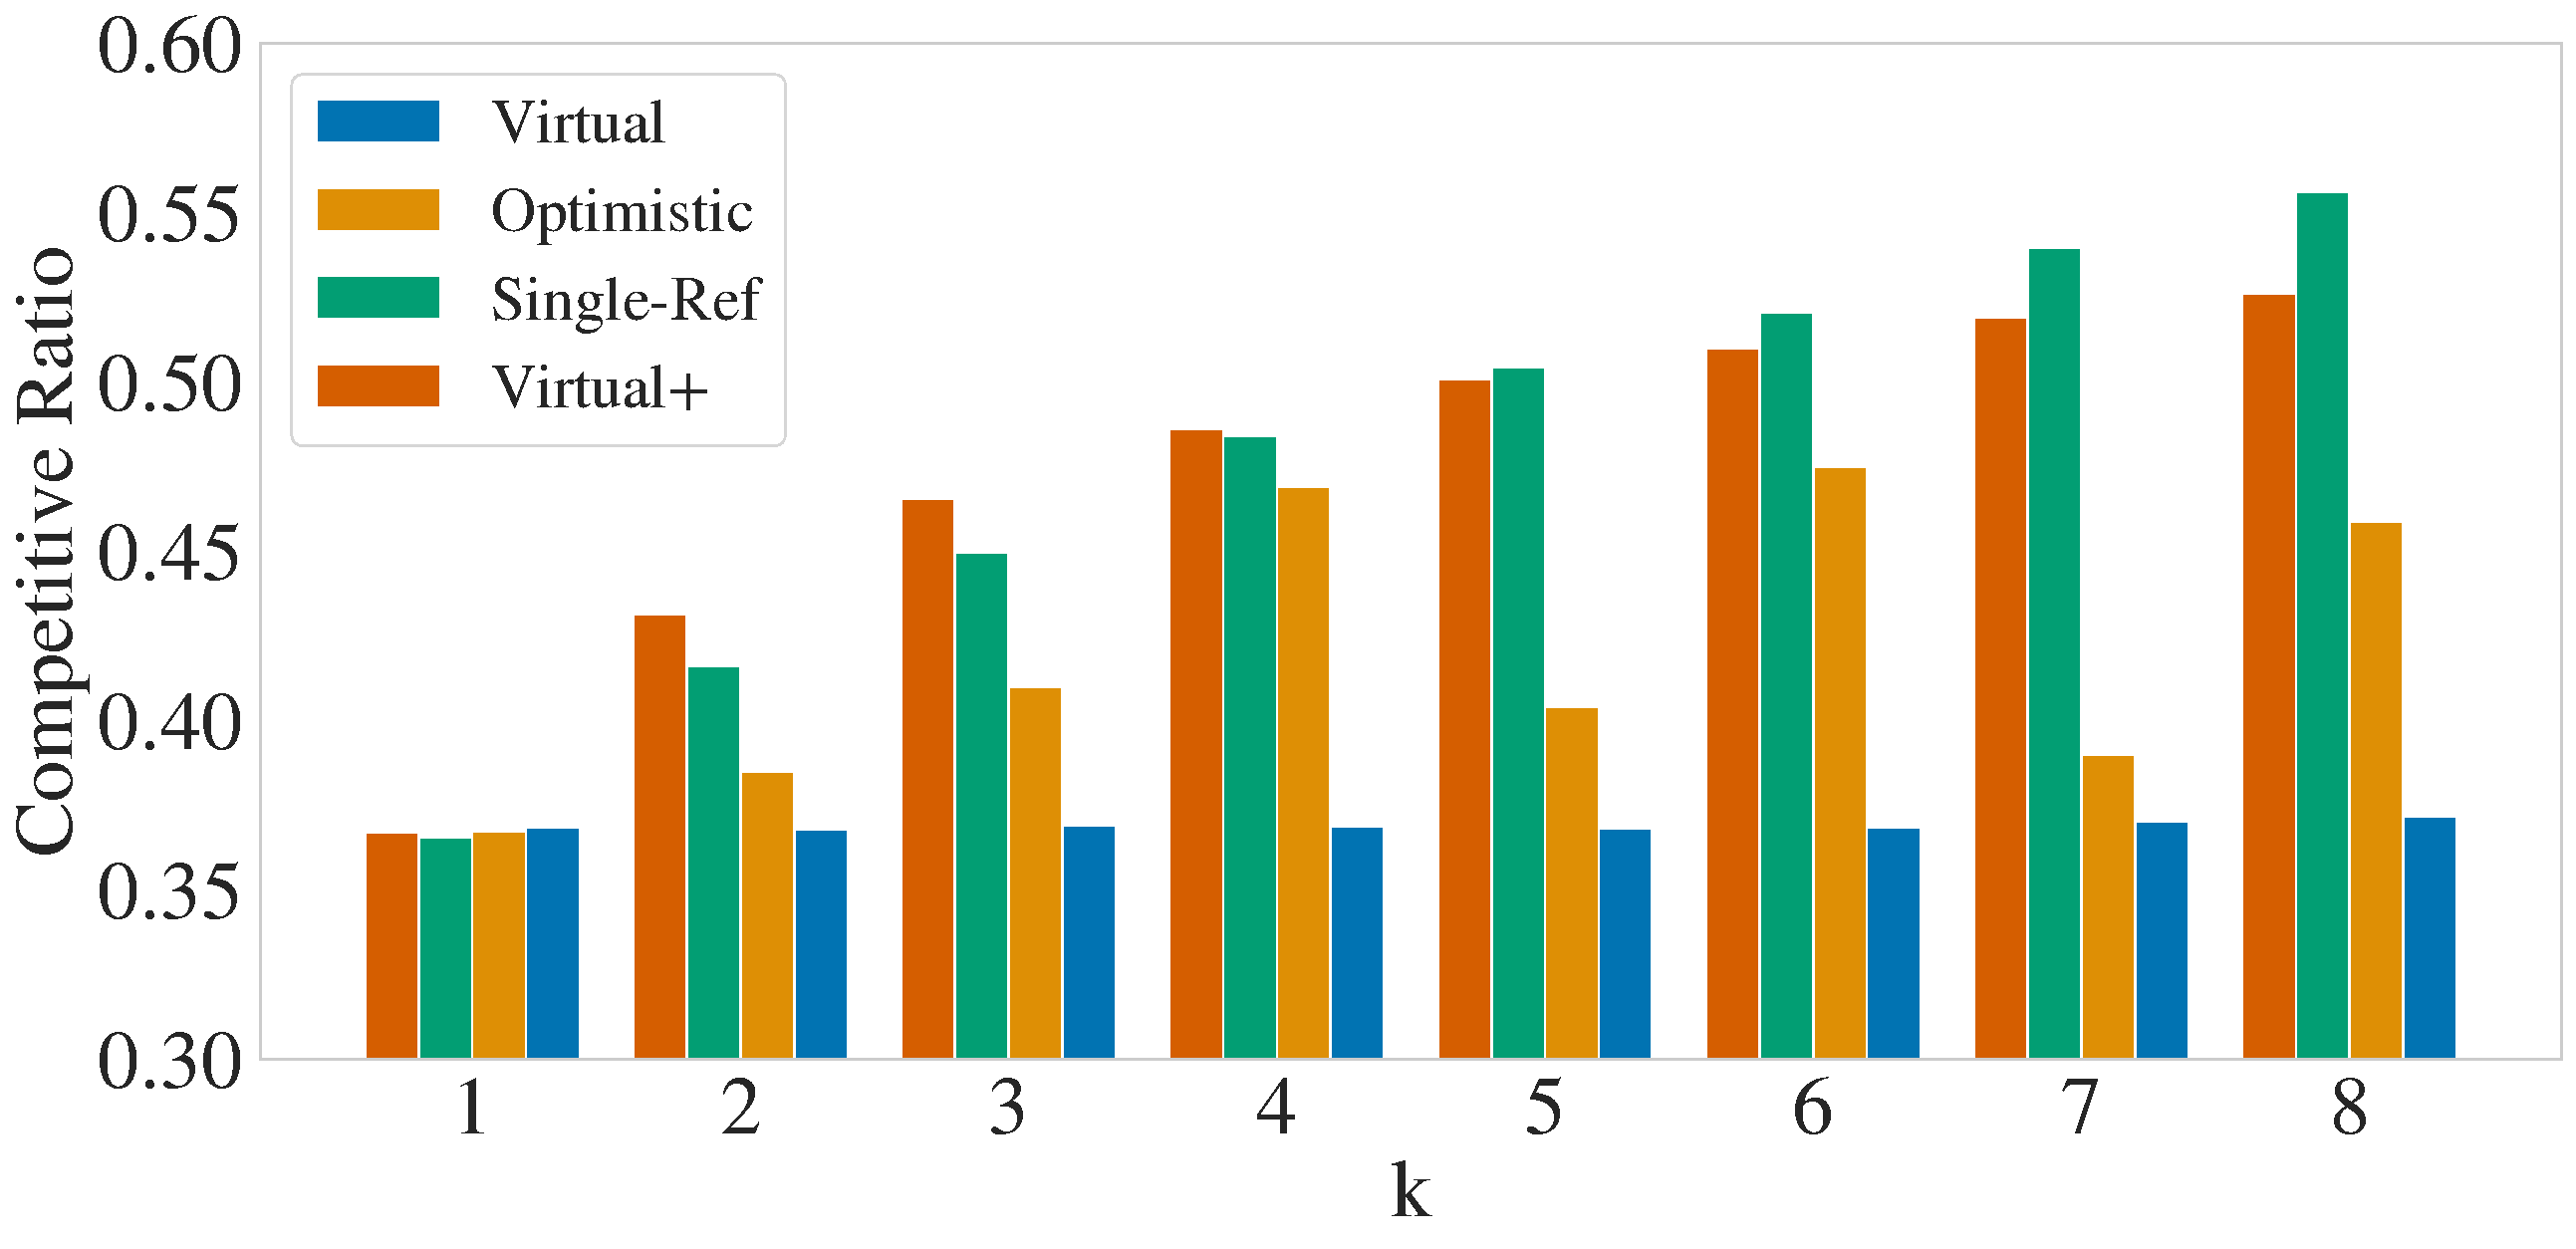
\includegraphics[width=1.01\linewidth]{Figures/Competitive_Ratio3Bar8-Var-10.pdf}
    % \vspace{-15pt}
    \caption{Estimation of the competitive ratio of online algorithms in the stochastic $k$-secretary problem with $\sigma^2=10$.}
    \label{fig:synthetic_data}
\end{figure}
\end{minipage}
\hfill
\begin{minipage}[t]{.48\textwidth}
\vspace{0pt}  
    \begin{algorithm}[H]
    \small
    \textbf{Inputs:} Permuted Datastream: $\mathcal{D}_\pi$, Online Algorithm: $\mathcal{A}$,  Surrogate classifier: $f_s$, Target classifier: $f_t$,  Attack method: \textsc{Att}, Loss: $\ell$,  Budget: $k$,  
    Online Fool rate: $F^{\mathcal{A}}_\pi=0$.
    \begin{algorithmic}[1]
    \FOR{$(x_i,y_i)$ in $\mathcal{D}_\pi$}
    \STATE $x_i' \leftarrow  \textsc{Att}(x_i)$ \hfill \COMMENT{// Compute the attack}
    \STATE $\mathcal{V}_i \leftarrow \ell(f_s(x_i'),y_i)$  \hfill \COMMENT{// Compute the estimate of $v_i$}
    \IF{$\mathcal{A}(\mathcal{V}_1,\ldots, \mathcal{V}_i,k) == \textsc{True}$}
    \STATE  $F^{\mathcal{A}}_\pi \leftarrow F^{\mathcal{A}}_\pi+\tfrac{\mathbf{1}\{f_t(x_i')\neq y_i\}}{k}$  \hfill\COMMENT{// Submit  $x_i'$ on $f_t$} 
    \ENDIF
    \ENDFOR
    \STATE \textbf{return:} $F^{\mathcal{A}}_\pi$ \hfill\COMMENT{//$\mathcal{A}$ always submits $k$ attacks} 
    \end{algorithmic}
     \caption{\small Online Adversarial Attack}
     \label{alg:online_adv_attack}
    \end{algorithm}
\end{minipage}

As illustrated for $k=1$ all algorithms roughly achieve the optimal $(1/e)$-deterministic competitive ratio in the stochastic setting. Note that the noise level, $\sigma^2$, appears to have a small impact on the performance of the algorithms (\S\ref{appendix:synthetic_additional_results}). 
This substantiates our result in Thm.~\ref{thm:stochastic_secretary} indicating that $C_n$-competitive algorithms only degrade by a small factor in the stochastic setting. For $k=2$, \algoname\ achieves the best competitive ratio validating our main result in Thm \ref{thm:K_2_theorem1}. \algoname\ continues to perform favorably for small values $k<5$ after which \textsc{Single-Ref} is superior. 
This was expected as we note that the hyperparameters in \textsc{Single-Ref}---e.g. $t$ and reference rank---are tuned offline for each value of $k$ by solving a separate combinatorial optimization problem while in \algoname\ we use the optimal $t$ for $k=2$ found in Eq.~\ref{eq:alpha_eqn}. We hypothesize that finding optimal thresholds for $k>2$ will further aid the performance of \algoname\ but leave this as future work.